\documentclass[greek]{beamer}
%\usepackage{fontspec}
%\newtheorem{definition}{Ορισμός}
\usepackage{amsmath,amsthm}
\usepackage{unicode-math}
\usepackage{xltxtra}
\usepackage{graphicx}
\usetheme{Warsaw}
\usecolortheme{seahorse}
\usepackage{hyperref}
\usepackage{ulem}
\usepackage{xgreek}
\usepackage{pgfpages}
%\setbeameroption{show notes on second screen}
%\setbeameroption{show only notes}

\setsansfont{Times New Roman}
\title{Η Πίεση και τα Μαθηματικά της}
\author[Λόλας, Ελευθεριάδης, Πετρίδης]{Κ. Λόλας\inst{1} \and Μ. Ελευθεριάδης\inst{2} \and Π. Πετρίδης\inst{3}}
\institute[]
{
  \inst{1}%
  10ο ΓΕΛ ΘΕΣ/ΝΙΚΗΣ (ΠΕ03)
  \and
  \inst{2}%
  32ο ΓΕΛ ΘΕΣ/ΝΙΚΗΣ (ΠΕ03)
  \and
  \inst{3}%
  ΓΕΛ ΧΑΛΑΣΤΡΑΣ (ΠΕ04.01)
}
\date{Λευκάδα, Οκτώβριος 2017}

\begin{document}
\begin{frame}
  \titlepage
\end{frame}

\section{Εισαγωγή}
\begin{frame}{Η Ανάγκη}
  \begin{itemize}
    \item Διαισθητικοί - Εμπειρικοί
    \item Μαθηματικό υπόβαθρο (?)
    \item Εμβάθυνση - Παράδοξα
  \end{itemize}
\end{frame}

\subsection{Πίεση}
\begin{frame}{Ορισμός}
  \begin{center}
    \begin{block}{Ορισμός (Β Γυμνασίου)}
      Πίεση ονομάζουμε το πηλίκο της δύναμης που ασκείται κάθετα σε μια επιφάνεια προς το εμβαδόν της επιφάνειας αυτής
    \end{block}
  \end{center}
  \note{Στο βιβλίο της Β Γυμνασίου υπάρχει ο ορισμός... \\ Δεν αφήνει περιθώρια για ερμηνεία...}
\end{frame}

\subsection{Εμπειρικά}
\begin{frame}{Πίεση - Εμπειρικά}
  \begin{figure}
    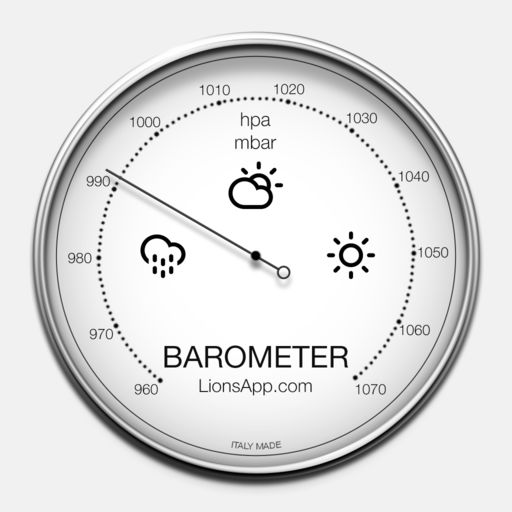
\includegraphics[scale=0.2]{barometer}
  \end{figure}
  \begin{itemize}
    \item<1-> Μονόμετρο
    \item<2-> \sout{Διανυσματικό}
  \end{itemize}
  \note{Διαισθητικά η πίεση είναι μονόμετρο... \\ Ένα βαρόμετρο τοίχου}
\end{frame}

\subsection{Μαθηματικά}
\begin{frame}{Πίεση - Μαθηματικά}
  \begin{itemize}
    \item<1-> $\vec{F}=p\vec{A}$
    \item<2-> $\displaystyle p=\frac{\vec{F}}{\vec{A}}$
  \end{itemize}
  \note{Αν η δύναμη είναι το παράγωγο μέγεθος τότε έχοντας και την επιφάνεια ως διάνυσμα... \\ Αν η πίεση είναι το παράγωγο...}
\end{frame}

\section{Διαίρεση}
\begin{frame}{Διαίρεση Διανυσμάτων}
  $$V \times V^* \to \mathbb{R}$$
  $$\frac{\vec{a}}{\vec{b}}=\frac{\vec{a}\cdot\vec{b}}{\left|\vec{b}\right|^2}$$
  \begin{itemize}
    \item<2-> Καλά ορισμένη πράξη
    \item<3-> Αρ.Επιμεριστική $\frac{\vec{a}+\vec{b}}{\vec{c}}=\frac{\vec{a}}{\vec{c}}+\frac{\vec{b}}{\vec{c}}$
    \item<4-> Προσεταιριστική $\frac{k\vec{a}}{\vec{c}}=k\frac{\vec{a}}{\vec{c}},\; k\in\mathbb{R}$
    \item<5-> \sout{Αντιμεταθετική}
    \item<6-> \sout{Προσεταιριστική}
    \item<7-> \sout{Ουδέτερο} - \sout{Αντίστροφο}
  \end{itemize}
  \note{Ιδιότητες διαίρεσης διανυσμάτων... \\
      Καλά ορισμένη πράξη \\
      Αρ.Επιμεριστική $\frac{\vec{a}+\vec{b}}{\vec{c}}=\frac{\vec{a}}{\vec{c}}+\frac{\vec{b}}{\vec{c}}$ \\
      Προσεταιριστική $\frac{k\vec{a}}{\vec{c}}=k\frac{\vec{a}}{\vec{c}},\; k\in\mathbb{R}$ \\
      \sout{Αντιμεταθετική} \\
      \sout{Προσεταιριστική} \\
      \sout{Ουδέτερο} - \sout{Αντίστροφο}}
\end{frame}

\section{Συμπεράσματα}
\begin{frame}{Διαίρεση Διανυσμάτων Συμπεράσματα}
  \begin{itemize}
    \item<1-> $\displaystyle\frac{\vec{a}+\vec{b}}{\vec{c}}=\frac{\vec{a}}{\vec{c}}+\frac{\vec{b}}{\vec{c}}$
    \only<2>{$$p(\vec{F_1}+\vec{F_2})=p(\vec{F_1})+p(\vec{F_2})$$}
    \item<3->$\displaystyle\frac{k\vec{a}}{\vec{c}}=k\frac{\vec{a}}{\vec{c}},\; k\in\mathbb{R}$
    \only<4>{$$p(k\vec{F})=kp(\vec{F})$$}
  \end{itemize}
  \note{Δύο ιδιότητες έχουν φυσική σημασία... \\ Η αριστερά επιμεριστική ως προς την πρόσθεση (η πίεση συνισταμένης=άθροισμα των επιμέρους) \\ Η πίεση μίας δύναμης πολλαπλασιασμένη με αριθμό είναι ο πολλαπλασιασμός της πίεσης με τον αριθμό}
\end{frame}

\section{Γενίκευση}
\subsection{Υδροστατική}
\begin{frame}{Υδροστατική Πίεση}
  \begin{block}{Παραδοχή}
    \begin{itemize}
      \item Ανεξάρτητη Επιφάνειας
      \item $ρ(z)=c$
      \item $g(z)=c'$
    \end{itemize}
  \end{block}
  Υδροστατική Εξίσωση $$\frac{dp}{dz}=-ρg$$
  \note{Η πρώτη εφαρμογή είναι η υδροστατική εξίσωση \\ Πολλές παραδοχές (Ανεξάρτητη της επιφάνειας - Ορισμός πίεσης σε σημείο, τα υγρά είναι ασυμπίεστα άρα η πυκνότητα είναι σταθερή, η επιτάχυνση της βαρύτητας είναι σταθερή σε μικρή διαφορά ύψους - Η θάλλασα είναι 11χλμ βαθιά το g είναι σταθερό) \\ Η Απόδειξη στην επόμενη διαφάνεια είναι για την ανεξαρτησία ως προς την επιφάνεια... \\ στην επόμενη είναι η απόδειξη της υδροστατικής}
\end{frame}

\subsubsection{Απόδειξη Σημείου}
\begin{frame}{Απόδειξη Ανεξαρτησίας ως προς Επιφάνεια}
  \begin{figure}
    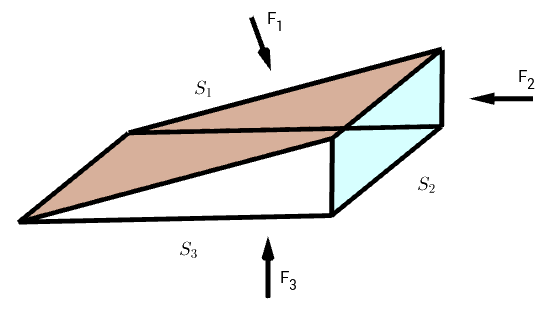
\includegraphics[scale=0.2]{Λευκάδα1}
  \end{figure}
  $$F_1 cosθ = F_3 \text{ και } F_1 sinθ = F_3$$
  Αντίστοιχα
  $$p_1 S_1 cosθ = p_3 S_3 \Rightarrow p_1=p_3$$ και $$p_1 S_1 sinθ = p_2 S_2 \Rightarrow p_1=p_2$$
\end{frame}

\subsubsection{Απόδειξη Υδροστατικής}
\begin{frame}{Απόδειξη Υδροστατικής}
  \begin{block}{Παραδοχή}
    \begin{itemize}
      \item $ρ(z)=c$
      \item $g(dz)=c'$
    \end{itemize}
  \end{block}
  \begin{columns}
    \column{0.75\textwidth}
      \begin{align*}
       \sum F_{z} & = 0 \Rightarrow  \\ F_{z1}-F_{z2} &=B \Rightarrow \nonumber\\
       \left(p_{z_0}-p_{z_0+dx} \right)dx\,dy&=\iiint_V ρg\,dx\,dy\,dz \Rightarrow \refstepcounter{equation} \nonumber \\
       -dp\,dx\,dy &= ρg\iiint_V dx\,dy\,dz \Rightarrow \nonumber\\
       -dp\,dx\,dy &= ρgdz\,dx\,dy \Rightarrow \frac{dp}{dz} =-ρg \nonumber
      \end{align*}
    \column{0.25\textwidth}
      \begin{figure}
        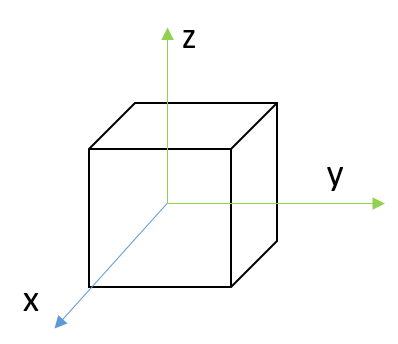
\includegraphics[scale=0.4]{Λευκάδα2}
      \end{figure}
  \end{columns}
\end{frame}

\subsection{Ατμοσφαιρική}
\begin{frame}{Ατμοσφαιρική Πίεση}
  \begin{block}{Παραδοχή}
    \begin{itemize}
      \item $g(z)=c$
      \item $T(z)=c'$
      \item $\displaystyle ρ=\frac{mp}{kT}$
    \end{itemize}
  \end{block}
  Εξίσωση Πίεσης $$p=p_0e^{-\frac{m}{kTg}z}$$
  \note{Παρατηρούμε πολλές παραδοχές :)... \\ H επιτάχυνση της βαρύτητας σταθερή \\ Η θερμοκρασία ως συνάρτηση του ύψους είναι σταθερή :( ... \\ Ισχύει η καταστατική εξίσωση (στην μορφή με την σταθερά Boltzman) άρα θεωρεί ιδανικό αέριο \\ στην επόμενη διαφάνεια η απόδειξη}
\end{frame}

\subsubsection{Απόδειξη}
\begin{frame}{Απόδειξη Ατμοσφαιρικής}
  \begin{gather*}
   \frac{dp}{dz}=-ρg \Rightarrow \\ \frac{dp}{dz}=-\frac{mp}{kT}g \Rightarrow \\ \frac{dz}{dp}=-\frac{kTg}{m}\frac{1}{p} \Rightarrow \\ z=-\frac{kTg}{m}\ln \frac{p}{p_0} \Rightarrow \\ p=p_0e^{-\frac{m}{kTg}z}
  \end{gather*}
\end{frame}

\subsection{Ρευστά}
\begin{frame}{Ρευστά}
  \begin{block}{Παραδοχή}
    \begin{itemize}
      \item Δεν υπάρχει τριβή με τα τοιχώματα
      \item Υγρό ασυμπίεστο
    \end{itemize}
  \end{block}
  Εξισώσεις
  \begin{itemize}
    \item<1-> Οριζόντιο σωλήνα: $\displaystyle \frac{ρv^2}{2}+p=c$
    \item<2-> Γενικά: $\displaystyle \frac{ρv^2}{2}+p+ρgh=c$
  \end{itemize}
  \note{Στα ρευστά περιπλέκονται πολλά \\ Η πίεση εξαρτάται από την ταχύτητα του ρευστού...\\πάλι έχει πολλές παραδοχές\\ 2 περιπτώσεις (η μία έχουμε μία ωραία απόδειξη που μπορεί να αντικαταστήσει του βιβλίου)}
\end{frame}

\subsubsection{Απόδειξη1}
\begin{frame}{Απόδειξη Ρευστών - Οριζόντιου}
  \begin{block}{Παραδοχή}
    \begin{itemize}
      \item Δεν υπάρχει τριβή με τα τοιχώματα
      \item Υγρό ασυμπίεστο
    \end{itemize}
  \end{block}
  \begin{gather*}
   F=ma \Rightarrow -Adp=ρV\frac{dv}{dt} \\
   -Adp=ρAdx\frac{dv}{dt} \Rightarrow -dp=ρv dv \\
   -\int_{p_1}^{p_2}dp=\int_{v_1}^{v_2}{ρv}dv \Rightarrow  p_2-p_1=\frac{1}{2}ρ(v_2^2-v_1^2) \\
   \frac{1}{2}ρv^2+p=c
  \end{gather*}
\end{frame}

\begin{frame}{Πίεση}
  \begin{gather*}
    p=\frac{\vec{F}}{\vec{A}}=\frac{\vec{F}\vec{A}}{\left| A \right|^2}
  \end{gather*}
\end{frame}

\begin{frame}[plain,c]
  \begin{center}
    \Huge Σας Ευχαριστούμε...
  \end{center}
\end{frame}

\end{document}
